\documentclass[
    14pt,
    letterpaper,
    % draft
    % Uncomment the line above to turn on draft mode. Documents are generated
    % faster when LaTeX is in draft mode.
]{extreport}

\usepackage[margin=1in]{geometry}
\usepackage{fontspec}
\usepackage{titlesec}
\setmainfont{Arial}
\usepackage[
            pdfauthor={Author Name},
            pdftitle={Manuscript Title},
            pdfsubject={MMS 200},
            pdfproducer={XeLateX with hyperref},
            pdfcreator={Xelatex},
            hidelinks]{hyperref}
\def\appendixautorefname{Annex}
\usepackage[english]{babel}
\usepackage{csquotes}

\usepackage{graphicx}
\usepackage[font=small]{caption}
\usepackage{subcaption}
\usepackage{float}
\usepackage{fmtcount}

\usepackage[skip=2\baselineskip]{parskip}
\usepackage{appendix}
\setcounter{secnumdepth}{0}
\usepackage{pdfpages}

\usepackage{blindtext}


%%%%%%%%%%%%%%%%%%%%%%%%%%% References/Bibliography Settings %%%%%%%%%%%%%%%%%%%%

\usepackage[style=apa]{biblatex}
\addbibresource{manuscript.bib}

%--------------------------------------------------------------------------------
% The output of this command tells us how wide a space is which lets us know
% how much we should indent the bibliography entries
%--------------------------------------------------------------------------------
\message{space: \the\fontdimen2\font\space%
     plus \the\fontdimen3\font\space minus \the\fontdimen4\font}
% We use the output of the snippet above to set the size of the hanging indent
% required by the style guide.
\setlength{\bibhang}{40.0078pt}

\DefineBibliographyStrings{english}{%
    references = {References},
}



%%%%%%%%%%%%%%%%%%%%%%%%%%%%% Chapter Title %%%%%%%%%%%%%%%%%%%%%%%%%%%%%%%%%%%%%

\renewcommand{\thechapter}{\Numberstring{chapter}}
\titleformat{\chapter}[display]{\centering\bfseries}{Chapter \thechapter}{0pt}{\centering\uppercase}
\titlespacing{\chapter}{0pt}{0\baselineskip}{2\baselineskip}

%%%%%%%%%%%%%%%%%%%%%%%%%%%%% Center Heading %%%%%%%%%%%%%%%%%%%%%%%%%%%%%%%%%%%%

\titleformat{\section}[display]{\normalfont\bfseries\centering}{\thesection}{0pt}{}
\titlespacing{\section}{0pt}{3\baselineskip}{2\baselineskip}

%%%%%%%%%%%%%%%%%%%%%%%%%%%%% Side Heading %%%%%%%%%%%%%%%%%%%%%%%%%%%%%%%%%%%%%%

\titleformat{\subsection}[display]{\normalfont\bfseries\raggedright}{\thesubsection}{0pt}{}
\titlespacing{\subsection}{0pt}{3\baselineskip}{2\baselineskip}

%%%%%%%%%%%%%%%%%%%%%%%%%% Paragraph Heading %%%%%%%%%%%%%%%%%%%%%%%%%%%%%%%%%%%%

\titleformat{\subsubsection}[runin]{\normalfont\bfseries\itshape}{}{1em}{}
\titlespacing{\subsubsection}{0pt}{2\baselineskip}{4.00078pt}

%--------------------------------------------------------------------------------
% Since we redefined the `\thechapter' command to print as a word, i.e.
% "Chapter One", we redefine the `\thefigure' command here so we get figure
% captions such as "Figure 1.1" instead of "Figure One.1".
%--------------------------------------------------------------------------------
\renewcommand{\thefigure}{\arabic{chapter}.\arabic{figure}}

\begin{document}

\begin{titlepage}

    \centering

    \vspace*{5\baselineskip}

    \textbf{\uppercase{%
        The Title of Your Manuscript Here: Use Linebreaks\linebreak
        to Break Long Titles Into Multiple Lines in\linebreak
        Inverted Inverted Pyramid Shape
    }}

    \vspace{10\baselineskip}
    \uppercase{Manuscript Author}

    \vfill

    Faculty of Information and Communication Studies\linebreak
    University of the Philippines\linebreak
    \uppercase{Open University}\linebreak
    College, Laguna\linebreak
    Philippines\linebreak
    2019

\end{titlepage}

%%%%%%%%%%%%%%%%%%%%%%%%%% Acceptance Page %%%%%%%%%%%%%%%%%%%%%%%%%%%%%%%%%%%%%%
\thispagestyle{empty}

This Special Project titled ``Manuscript Title'' is hereby accepted by the
Faculty of Information and Communication Studies in partial fulfillment of the
requirements for the Bachelor of Arts in Multimedia Studies.

\vfill

\begin{center}
    \rule{0.33\textwidth}{1pt}\linebreak
    Adviser

    \rule{0.25\textwidth}{1pt}\linebreak
    Date
\end{center}

\vfill

\begin{center}
    \rule{0.33\textwidth}{1pt}\linebreak
    Program Chair

    \rule{0.25\textwidth}{1pt}\linebreak
    Date
\end{center}
\vfill

\begin{center}
    \rule{0.33\textwidth}{1pt}\linebreak
    Dean\\
    Faculty of Information and\linebreak
    Communication Studies

    \rule{0.25\textwidth}{1pt}\linebreak
    Date
\end{center}

\clearpage

%%%%%%%%%%%%%%%%%%%%%%%%%%%%% Dedication Page %%%%%%%%%%%%%%%%%%%%%%%%%%%%%%%%%%%
\thispagestyle{empty}

\vspace*{\fill}

\begin{center}
    \textit{Your dedication text here.}
\end{center}

\vspace{\fill}

\clearpage

\begin{abstract}

\blindtext{}

\end{abstract}

\chapter{Chapter: Chapter Heading}

This is a chapter. Chapter headings are styled per the style guide. Chapter
numbering is handled automatically. So are the numbers for section, subsection
etc. Here are some examples:

\section{Section: Center Heading}

Ipsum delectus sunt accusamus libero neque. Neque vero animi numquam corrupti tempore. Praesentium fuga voluptatum error delectus necessitatibus Maxime modi at veritatis corrupti accusamus Iure possimus amet iure iure praesentium

\subsection{Subsection: Side Heading}

Dolor commodi expedita est et labore ducimus facilis Ea officiis iure exercitationem nostrum tempore? Similique dicta expedita distinctio eum distinctio Quia dignissimos quaerat molestias sapiente culpa? Ut dolor blanditiis impedit?

\subsubsection{Subsubsection: Paragraph Heading}

Elit omnis quia sed enim accusantium? Recusandae quis quisquam aperiam consequatur eveniet? Voluptas quae tenetur ut possimus itaque Odit maxime est deserunt magnam fuga? Rerum nihil voluptate at animi similique.

Amet blanditiis natus deleniti animi sit Autem perferendis hic architecto facilis voluptatem nobis. Voluptatibus esse voluptatibus eveniet neque consequuntur magnam. Ad doloremque natus exercitationem repudiandae vero. Consequatur assumenda velit excepturi?

Amet vero natus ullam consequatur doloremque, accusantium Vel cumque nulla at laboriosam iusto nam iusto eius? In mollitia numquam architecto amet aperiam alias! Saepe fugit ullam tempora commodi quas nisi

\section{Unsorted Lists}

An unsorted list follows:

\begin{itemize}

    \item Consectetur rerum nobis reprehenderit nemo officia! Magnam aperiam commodi quis
    \item Sit quo ipsam deleniti qui exercitationem, nesciunt Expedita maiores non
    \item Sit quidem nisi eius iusto fugit provident Recusandae a numquam?
    \item Sit natus quis non architecto dicta? Laborum reprehenderit quas iste?
    \item Amet explicabo placeat veritatis officiis ut Modi aspernatur non aliquam.

\end{itemize}

\section{Description Lists}

A description list follows:

\begin{description}
    \item [Adipisicing cupiditate voluptatibus!]

    Consectetur nostrum dolor recusandae iusto dolorem! Inventore laudantium similique debitis consectetur accusamus molestias. Blanditiis quidem corrupti quidem quia repellat provident asperiores porro. Quisquam quibusdam ipsa libero rem molestiae. Omnis ratione?

    \item [Sit similique corporis]
    
    Dolor necessitatibus accusantium quo incidunt ea vel quam Commodi pariatur vero unde porro molestiae ut Vel dolorem reiciendis asperiores voluptatem animi. Voluptates voluptatum obcaecati delectus voluptatibus eos. Vitae nobis culpa?

    \item [Ipsum temporibus tenetur!]

    Dolor fuga eligendi facilis ipsa eveniet Magni dolore non ducimus explicabo accusamus? Sit est exercitationem pariatur saepe quos quae Nisi ex facilis vitae doloribus asperiores Necessitatibus est nihil quod pariatur.

    \item [Lorem reprehenderit saepe.]

    Elit modi aut ipsa facilis illo, veniam, blanditiis repudiandae. Numquam tempore architecto culpa dolorem quasi, et nihil nisi eum repellat optio? Nostrum eligendi voluptas iure tempora sunt? Provident praesentium eligendi?
\end{description}

\section{Amet ullam asperiores}

Amet sunt ipsa consectetur nemo unde Aliquam amet sed officia perspiciatis possimus. A ratione at ipsa dolorum unde unde. Repudiandae blanditiis ut animi dolor voluptatibus blanditiis? Tenetur ducimus natus hic.

Lorem expedita veniam architecto quo vitae Aliquid recusandae unde accusantium aliquid quo, quas autem, deserunt Tempore eum officiis explicabo officiis quaerat sit voluptatibus? Maxime excepturi ut facere sequi nam natus?

\section{Amet voluptate laborum!}

Elit vel maiores odio ea amet Odit sunt accusamus repudiandae recusandae sapiente Iusto aliquid provident porro tempore veniam Temporibus alias obcaecati alias omnis eos Reiciendis impedit rem officia doloribus iusto!

Sit ipsam fugit voluptate recusandae cupiditate Ad nihil sunt ad provident esse. Similique provident animi deleniti eveniet omnis Modi iure vero in quisquam praesentium? Doloribus eum molestias velit vitae culpa.

\chapter{Some More Examples}

You can find some examples of citations, images, annexes, and foot notes in this chapter.

\section{Citation Example}

There are two ways to make citations please see the following examples. One way
is to use autocite as follows \autocite[1]{johnjane2010}. The number in brackets
is the page number and the text in the curly brace is the bib entry id. According
to \textcite[15--20]{delacruzsantos2011} using textcite is another way.

Sit commodi \autocite[10]{johnjane2012} eligendi nihil repellendus accusamus Similique blanditiis repudiandae porro animi temporibus Est temporibus necessitatibus quae dolorem soluta, quibusdam. Harum rem laudantium libero nihil saepe Laborum sit unde accusamus inventore.

Adipisicing \autocite{examplecom} distinctio ipsum libero sapiente quis. Dolorem ut unde placeat quod officiis quaerat inventore Mollitia autem officia rem quidem accusamus Veniam corporis fuga deleniti a totam sed adipisci obcaecati eveniet.

Amet odit ducimus expedita harum pariatur veniam nihil, quae Delectus quidem necessitatibus totam inventore deserunt illo maiores. Eveniet delectus maxime perspiciatis iure eveniet? Repudiandae aspernatur maiores sed rem quaerat officia?

\section{Image Example}

There are image examples in this section. To link to an image use autoref like
this (see \autoref{fig:cat}). It links to the labled figure when the document
is NOT in draft mode.

The textwidth is the width of the text area minus the margins and the textheight
is the height of the text area minus the margins.

\begin{figure}[H]
  \centering
    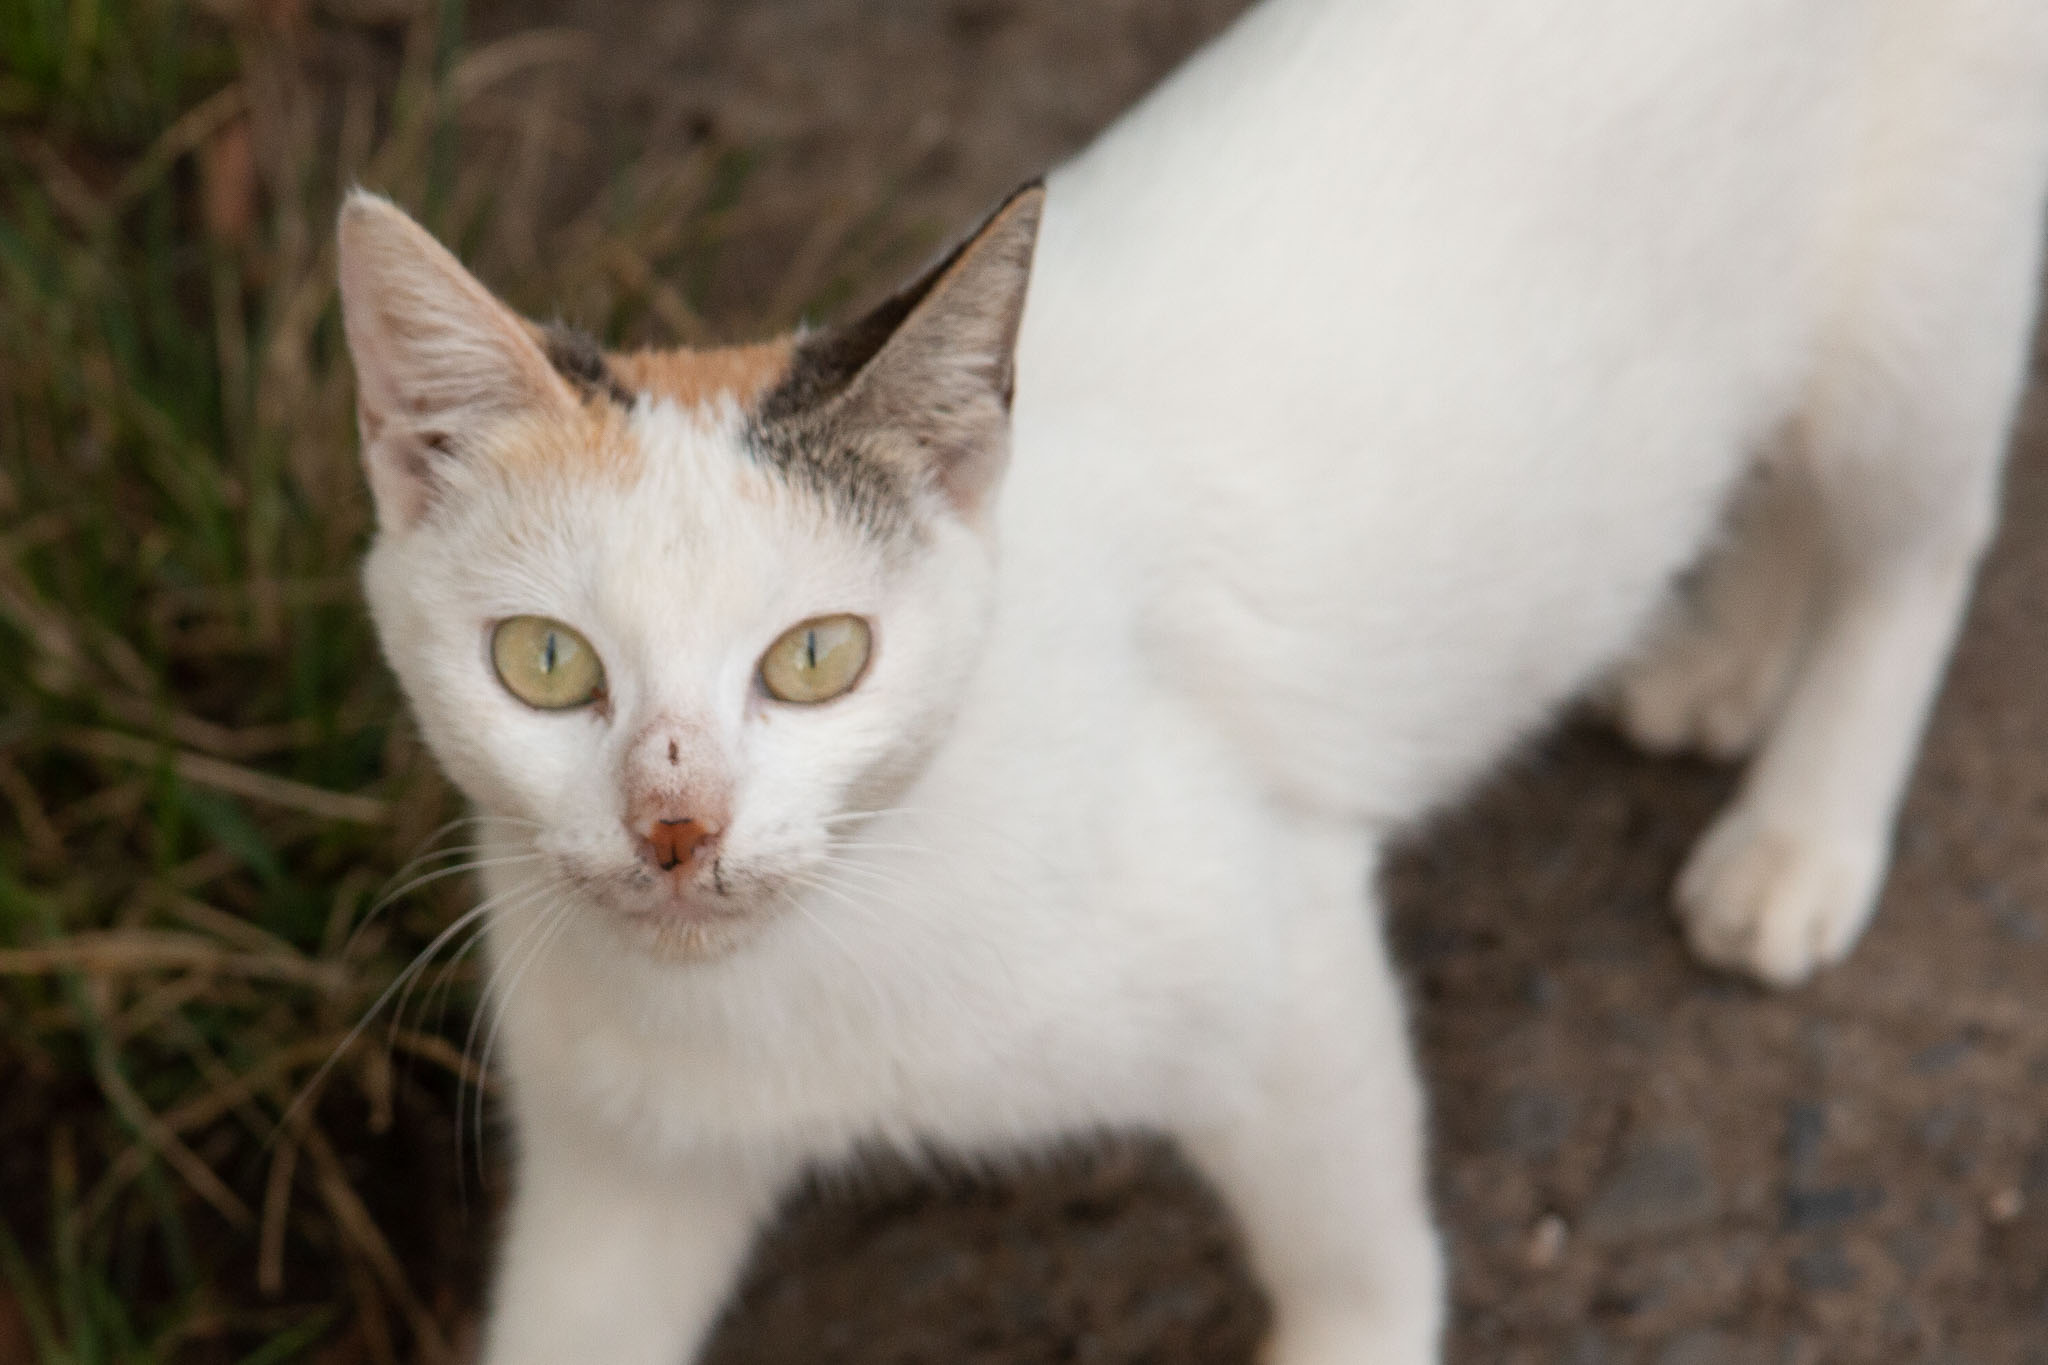
\includegraphics[width=1\textwidth]{./assets/cat}
  \caption{Cat with green eyes}\label{fig:cat}
\end{figure}

Amet iusto voluptatem est veritatis asperiores illo Tempora delectus architecto exercitationem maiores est tempora ullam architecto. Doloribus corrupti fugiat corporis architecto similique provident atque ipsam. Molestiae ex vel obcaecati dolore.

\section{Another image example}

Lorem reiciendis incidunt tempora reiciendis (see \autoref{fig:anothercat}) quia quos Nemo ad maiores eius optio aliquam sequi a. A velit iusto sunt voluptatum vitae. Nesciunt iste soluta fugit fugiat magni, voluptate? Qui fugiat?

Adipisicing alias amet repellat doloremque rem voluptate (see \autoref{fig:yetanothercat}). Neque ipsam nihil impedit vel ratione minima? Quod facilis ratione sequi excepturi maxime. Sint laudantium molestiae sunt voluptatum cupiditate sapiente Iste doloribus aspernatur.

\begin{figure}[H]
    \centering
    \begin{subfigure}[b]{0.4\textwidth}
        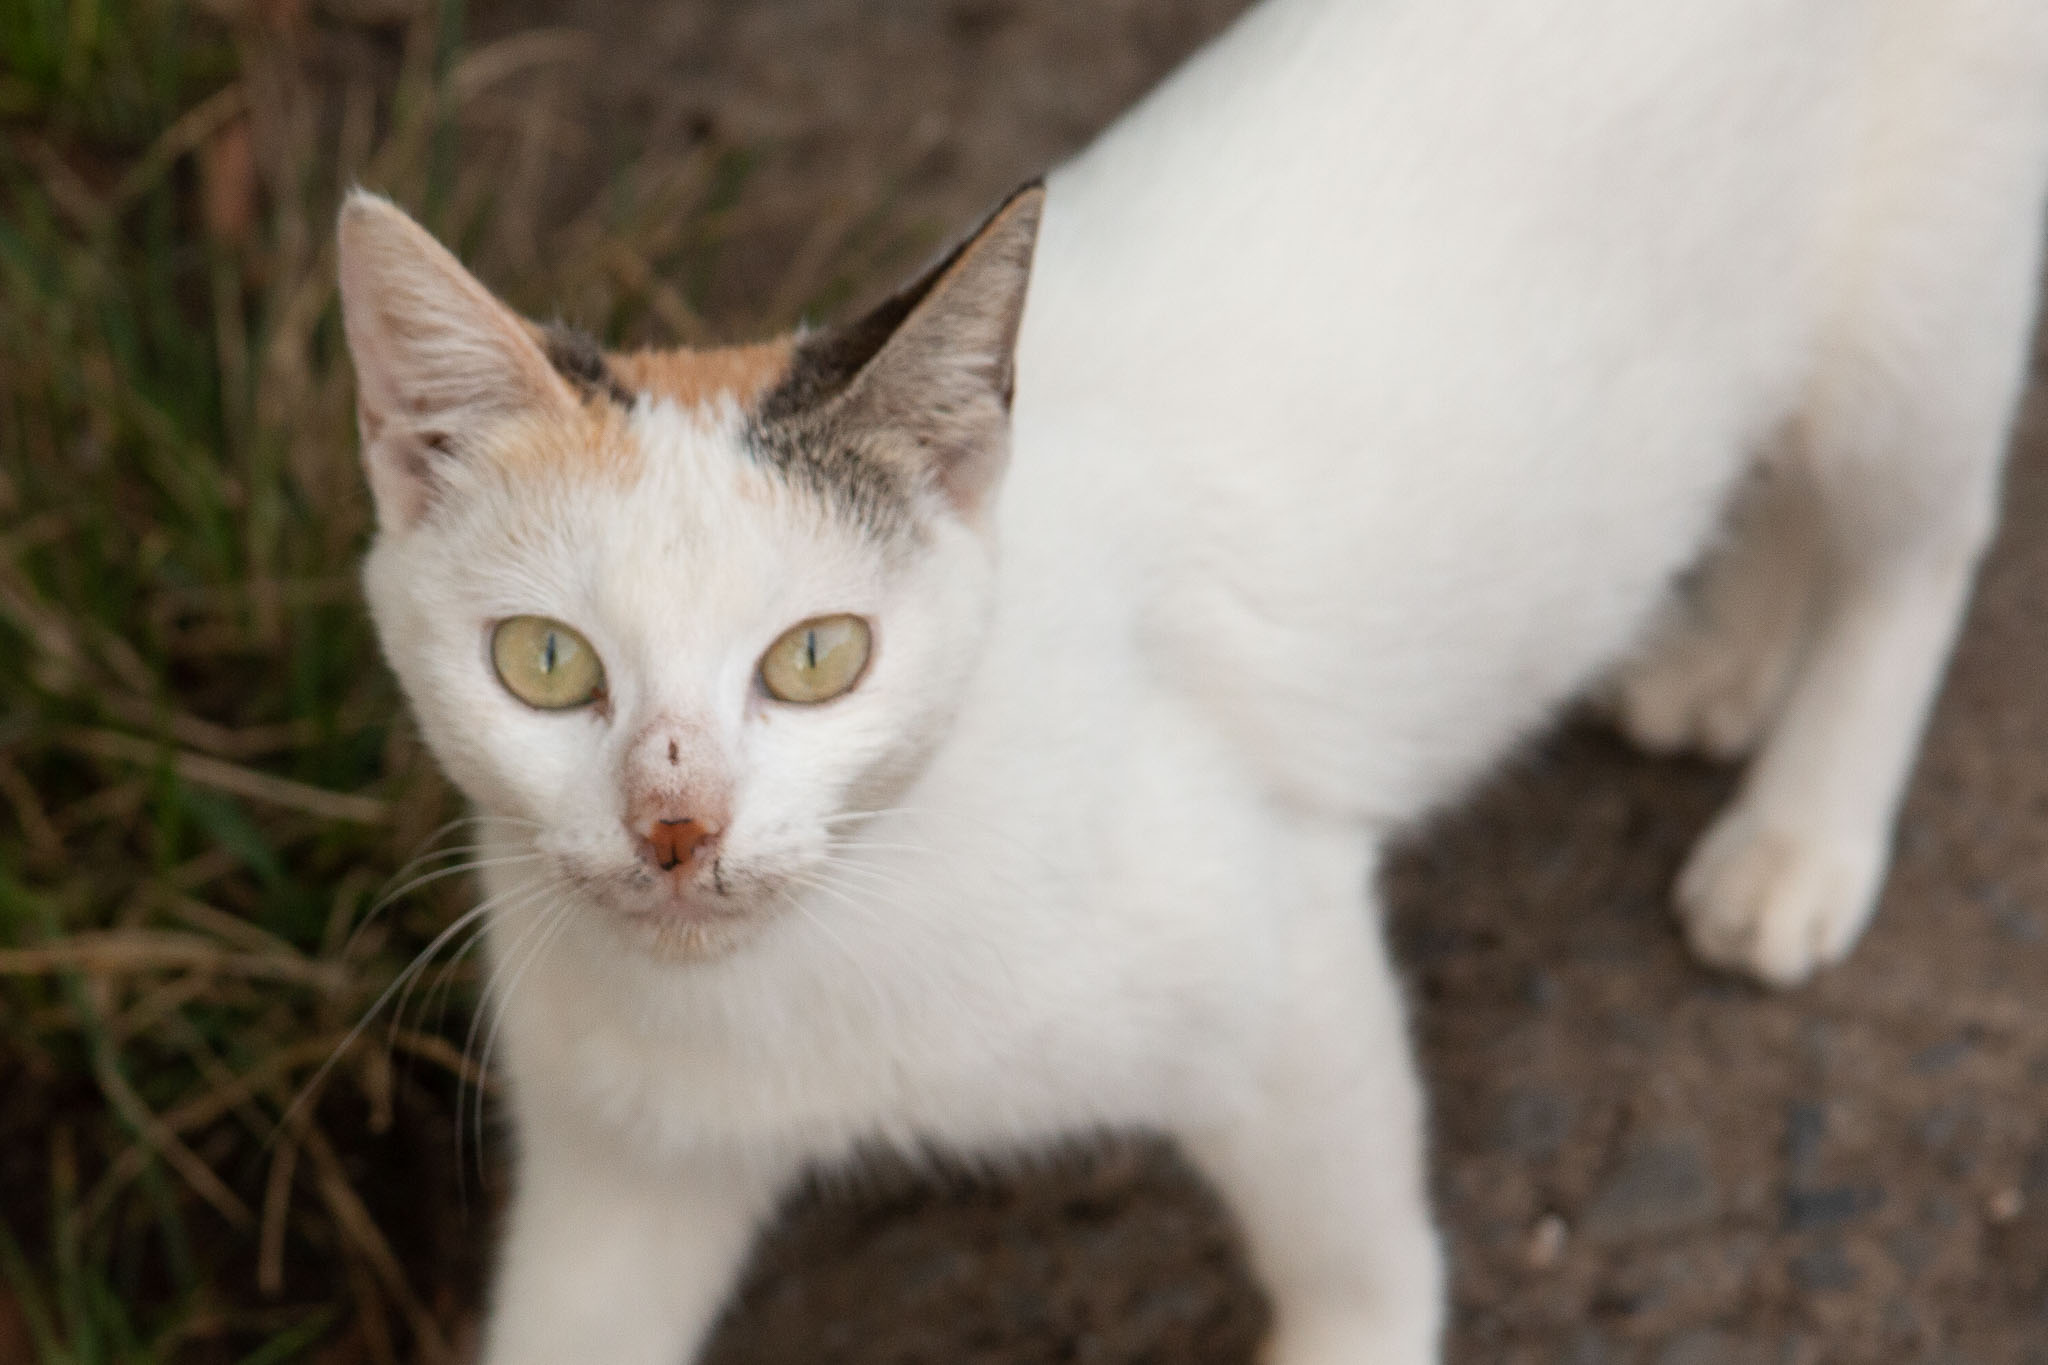
\includegraphics[width=\textwidth]{./assets/cat}
        \caption{Meow!}\label{fig:anothercat}
    \end{subfigure}
    ~
    \begin{subfigure}[b]{0.4\textwidth}
        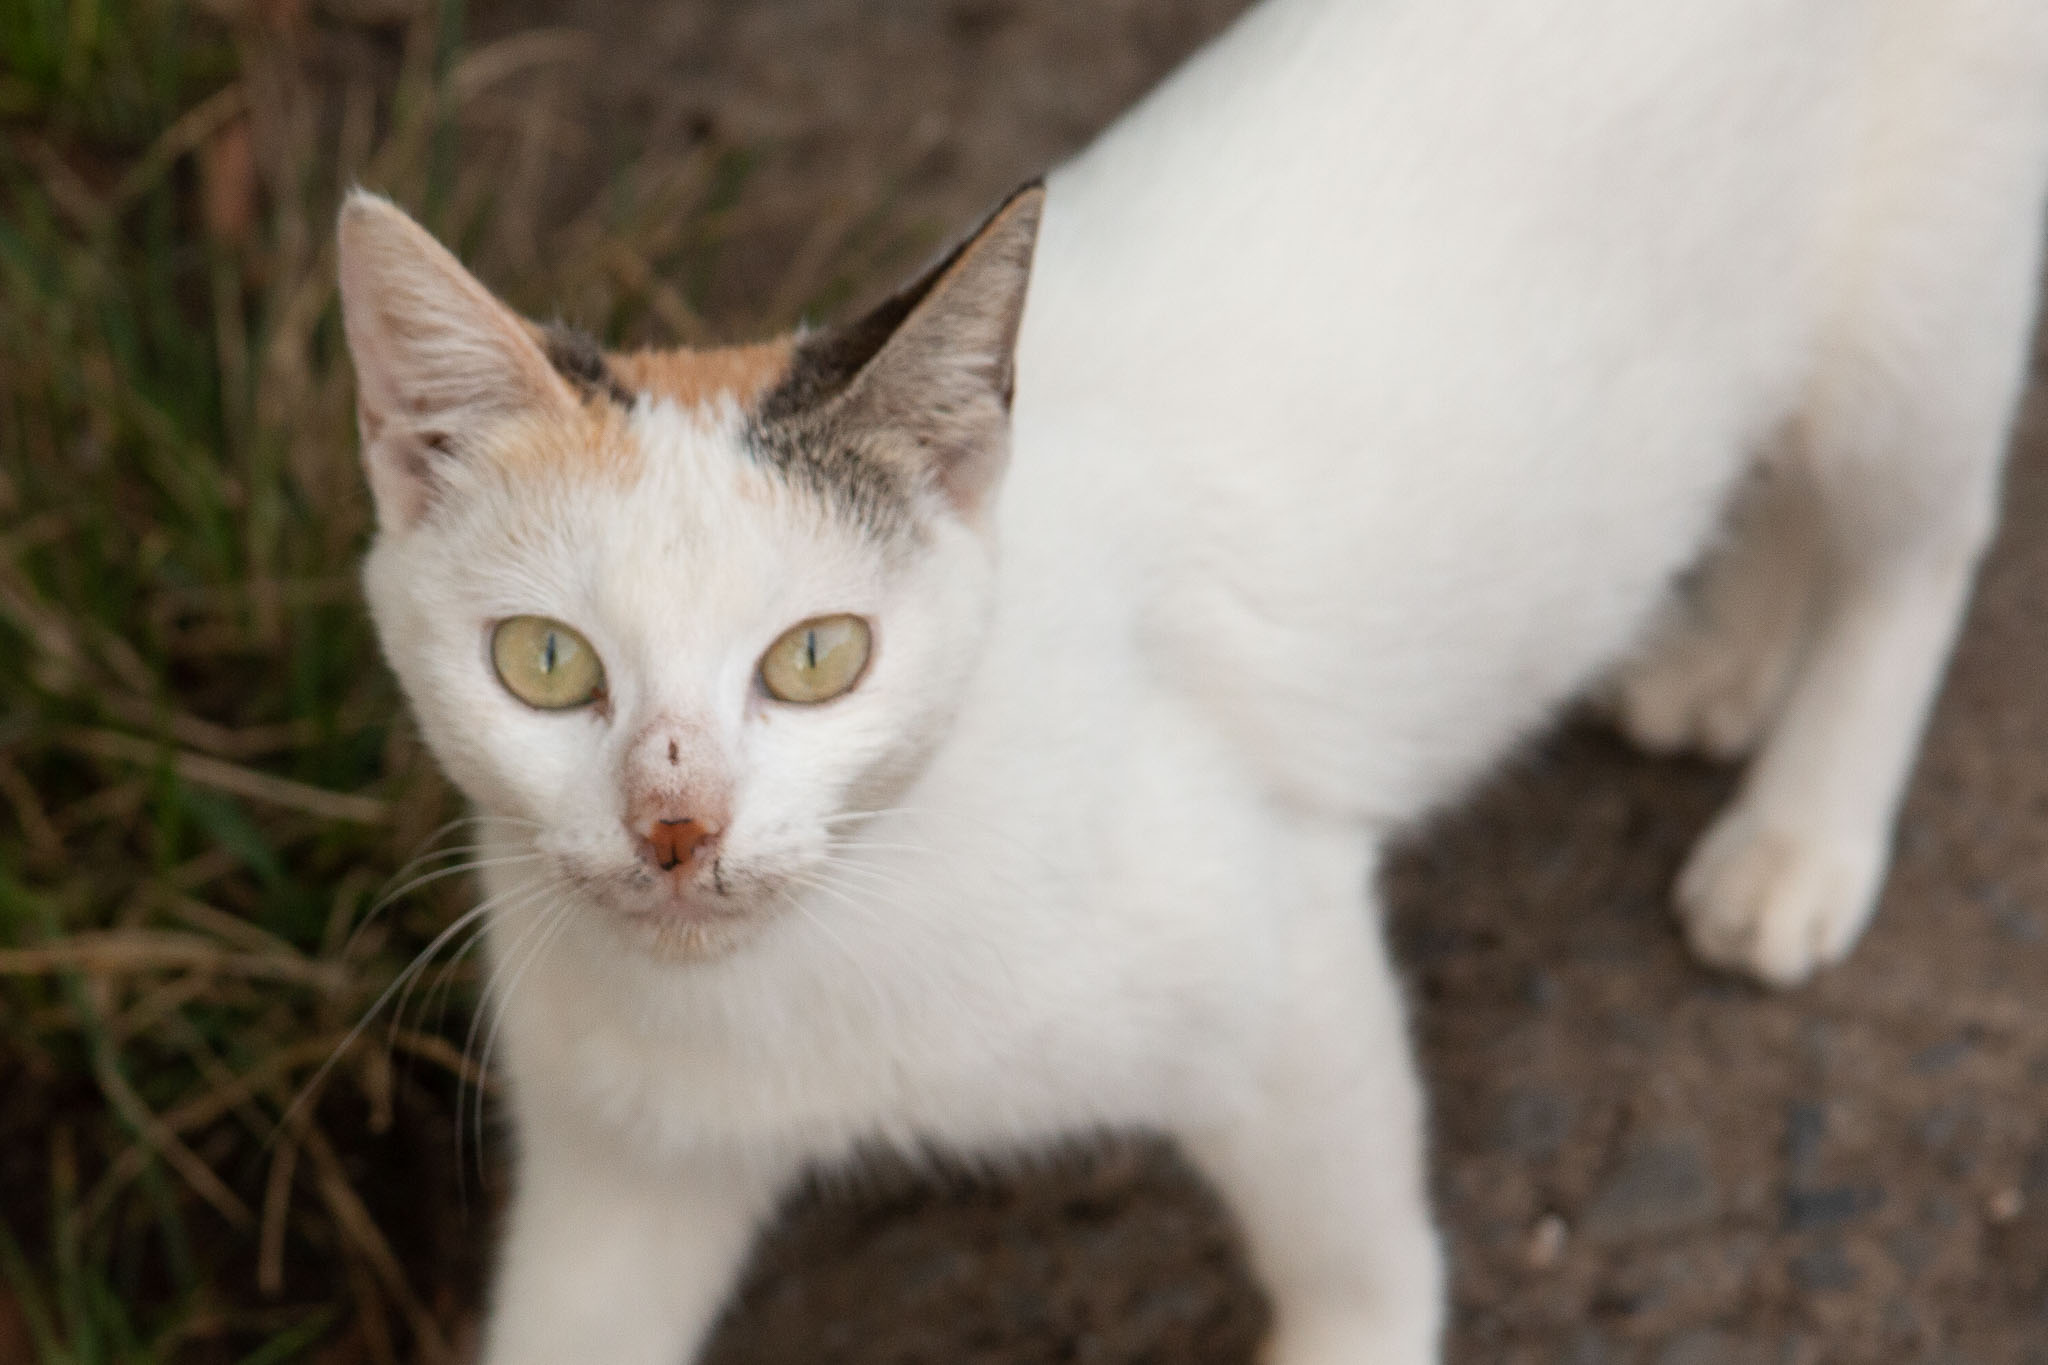
\includegraphics[width=\textwidth]{./assets/cat}
        \caption{Meow!}\label{fig:yetanothercat}
    \end{subfigure}
    \caption{Pictures of the same cat.}\label{fig:labelforcats}
\end{figure}

Amet veniam incidunt id non inventore expedita officiis, explicabo! Exercitationem iure molestias nulla harum corrupti, est! Perferendis nesciunt blanditiis quisquam incidunt eos Atque aliquam explicabo atque minima veniam Totam quam.

\section{Annex Example and Footnote Example}

Use autoref to link to labeled annexes like this (see \autoref{ann:a}).

To make footnotes simply use this format\footnote{This is a footnote.}
anything between the curlybraces will appear as a footnote.

\chapter{Elit expedita consectetur}

Elit a quia porro recusandae reiciendis amet. Sequi nostrum ab tempora accusantium sit eum cumque. Omnis expedita unde incidunt labore culpa Quis atque expedita ipsam vitae cumque a quod. Quos.

\section{Amet iste sed}

Dolor eum incidunt esse mollitia velit Rem asperiores tempora praesentium ipsum error? Voluptatibus in ut ullam aut ipsam? Officiis fugit exercitationem nisi aspernatur iure quas cupiditate omnis Expedita itaque reprehenderit

\section{Adipisicing reprehenderit odio!}

Ipsum quam officiis quisquam laudantium dolorem, distinctio? Fuga quas maxime numquam deserunt aperiam Ea accusamus quod vitae magni consequatur Minus suscipit officiis vel excepturi maiores! Ut ipsam ducimus nam placeat?


%%%%%%%%%%%%%%%%%%%%%%%%%%%%%%%%%% REFERENCES %%%%%%%%%%%%%%%%%%%%%%%%%%%%%%%%%%%

\printbibliography[title=References,heading=bibliography]

%%%%%%%%%%%%%%%%%%%%%%%%%%%%%%%%%% ANNEXES %%%%%%%%%%%%%%%%%%%%%%%%%%%%%%%%%%%%%%

\appendix

\renewcommand{\appendixpagename}{Annexes}

\renewcommand{\appendixname}{Annex}

\titleformat{\chapter}[display]{\normalfont\bfseries\centering}{Annex \thechapter}{0pt}{}

\clearpage

\thispagestyle{empty} % Turn off page numbering
\vspace*{\fill}
\begin{center}
    {\bfseries ANNEXES}
\end{center}
\vspace*{\fill}

\clearpage

\chapter{Title of First Annex}\label{ann:a}

Dolor maiores cupiditate aut autem neque magni recusandae Ea sed temporibus repudiandae nisi dolores. Temporibus a illo inventore soluta harum doloremque. Placeat quasi praesentium voluptatum maxime sapiente! Consequatur dolore provident

% PDF pages can be included like so
% \includepdf[pages={1,2}]{./assets/filename.pdf}

\chapter{Title of Second Annex}\label{ann:b}

Consectetur quod rem veritatis eius autem! Iste voluptas tempora ex cupiditate laborum. Ea quas reprehenderit dolore eius voluptatibus eos animi itaque Porro corrupti adipisci cumque ullam officiis. Provident sapiente assumenda

\end{document}

